\chapter{Arhitektura i dizajn sustava}
		\graphicspath{{./slike/}}
\noindent Arhitektura sustava može se podijeliti na tri glavna podsustava, a to su: web preglednik, web poslužitelj i baza podataka.

\begin{itemize}
	
	\item  \textbf{Web preglednik} je program koji služi za pristup web stranicama. Putem web preglednika, korisnik šalje zahtjeve za resursima (npr. HTML kod web stranice) ili šalje podatke (npr. putem neke forme), web preglednik dohvaća te datoteke s web poslužitelja, a potom ih interpretira i prikazuje na ekranu korisnika ili ih pohranjuje na poslužitelju. 
	
	\item \textbf{Web poslužitelj} glavni je dio web aplkacije. To je namjensko računalo ili softver koji šalje i prima podatke od mnogostrukih klijenata. Komunikacija s klijentima (korisnicima i bazom podataka) odvija se preko HTTP protokola. Na korisnikov zahtjev, web preglednik dohvaća resurse i vraća u obliku HTML dokumenta ili obrađuje podatke predane u formi te ih sprema u bazu podataka. 

	\item \textbf{Baza podataka} koristi se za pohranjivanje podataka sustava. Web aplikacija u svom radu vrlo često komunicira s bazom te iz nje dohvaća podate ili ih u nju sprema. 
\end{itemize}
Pri oblikovanju aplikacije koristili smo MVC (Model-View-Controller) obrazac softverske arhitekture.
Po principu MVC-a, aplikaciju dijelimo na tri komponente:	

\begin{itemize}
	
	\item \textbf{Model} je glavna komponenta sustava. Predstavlja strukturu podataka (Java objekti) i njihovu funkcionalnost.
	
	\item \textbf{View} odlučuje kako će se dohvaćeni podaci reprezentirati.
	
	\item \textbf{Controller}  zaprima zahtjeve za resursima (HTTP zahtjevi) od klijenta koje prilagođava i prosljeđuje Modelu ili Viewu. 
	
\end{itemize}
Programski jezik kojeg smo odabrali za izradu backenda naše aplikacije je Java zajedno sa Spring Boot radnim okvirom u razvojnom okruženju Intellij, a u izradi frontenda koristili smo jezike JavaScript i TypeScript te biblioteke React, Redux i Axios uz razvojno okruženje Visual Studio Code. 







	
		

		

				
		\section{Baza podataka}
			
			
		\textit {\normalfont} U ovom projektu koristit ćemo relacijsku bazu u kojoj će gradivne jedinke biti entiteti, definirani imenom i skupom atributa. Zadaća baze je pohrana podataka o satelitima, linkovima, baznim stanicama i korisnicima. Sukladno time entiteti koje ćemo kreirati su:

        \begin{itemize}
            \item User
            \item Satellite
            \item Transmitter
            \item Link
            \item Station
            \item Antenna
            \item Message
        \end{itemize}
		
			\subsection{Opis tablica}
			

				\textbf{User} {\normalfont} Ovaj entitet sadrži podatke o korisniku                aplikacije. Njegovi atributi su:\newline userId (PRIMARY KEY), username, email,         password i roleName.
                    Ovaj entitet u vezi je \emph{One-to-Many} s entitetom Satellite preko atributa userId, u vezi \emph{One-to-Many} s entitetom Link preko atibuta userId i u vezi \emph{One-to-Many} s entitetom Message preko atributa userId.
				
				
				\begin{longtblr}[
					label=none,
					entry=none
					]{
						width = \textwidth,
						colspec={|X[6,l]|X[6, l]|X[20, l]|}, 
						rowhead = 1,
					} %definicija širine tablice, širine stupaca, poravnanje i broja redaka naslova tablice
					\hline \SetCell[c=3]{c}{\textbf{User}}	 \\ \hline[3pt]
					\SetCell{LightGreen}userId & INT	&  Jedinstveni brojčani identifikator, autogeneriran od strane baze  	\\ \hline
				\SetCell{LightBlue} username	& VARCHAR &  Jedinstveno korisničko ime\\ \hline 
					\SetCell{LightBlue} email & VARCHAR &  Jedinstvena email adresa \\ \hline 
					password & VARCHAR	&  Šifrirana lozinka\\ \hline 
                    roleName & VARCHAR & SUPER\_ADMIN (admin aplikacije), SATELLITE\_ADMIN (admin satelita) ili USER (običan korisnik)\\ \hline
				\end{longtblr}

                     \textbf{ Satellite} {\normalfont} Ovaj entitet sadrži podatke o satelitima u Zamljinoj orbiti. Njegovi atributi su: satelliteId (PRIMARY KEY), satName i satelliteStatus.
                    Ovaj entitet u vezi je \emph{Many-to-One} s entitetom User preko atributa userId, u vezi \emph{Many-to-Many} s entitetom Transmitter preko atributa satelliteId i transmId.

                    \begin{longtblr}[
					label=none,
					entry=none
					]{
						width = \textwidth,
						colspec={|X[6,l]|X[6, l]|X[20, l]|}, 
						rowhead = 1,
					} %definicija širine tablice, širine stupaca, poravnanje i broja redaka naslova tablice
					\hline \SetCell[c=3]{c}{\textbf{Satellite}}	 \\ \hline[3pt]
					\SetCell{LightGreen}satelliteId & INT	&  	Jedinstveni brojčani identifikator, autogeneriran od strane baze  	\\ \hline
					\SetCell{LightBlue} satName	& VARCHAR &   Naziv satelita\\ \hline 
					satelliteStatus & VARCHAR &  Active (dostupan/aktivan) ili inactive (nedostupan/neaktivan)\\ \hline  
				\end{longtblr}

                    \textbf{Transmitter} {\normalfont} Ovaj entitet sadrži podatke o transmiterima koji se nalaze na satelitu. Njegovi atributi su: transmId (PRIMARY KEY), transmFreq, transmMode, transmBaud i transmName.
                    Ovaj entitet u vezi je \emph{Many-to-Many} s entitetom Satellite preko atributa satelliteId i transmId i u vezi \emph{Many-to-One} s entitetom Link preko atributa linkId.
				
				
				\begin{longtblr}[
					label=none,
					entry=none
					]{
						width = \textwidth,
						colspec={|X[6,l]|X[6, l]|X[20, l]|}, 
						rowhead = 1,
					} %definicija širine tablice, širine stupaca, poravnanje i broja redaka naslova tablice
					\hline \SetCell[c=3]{c}{\textbf{Transmitter}}	 \\ \hline[3pt]
					\SetCell{LightGreen}transmId & INT	&  Jedinstveni brojčani identifikator, autogeneriran od strane baze  	\\ \hline
				transmFreq & VARCHAR & Frekvencija na kojoj transmiter može komunicirati\\ \hline
                    transmMode & VARCHAR & Radio-frekvencijska modulacija transmitera (oznaka za način kodiranja informacije u u radio-signalu)\\ \hline
					transmBaud & VARCHAR & Broj kodiranih informacija (definiranih modeom transmitera) koje se mogu promijeniti u jedinici vremena\\ \hline
                    \SetCell{LightBlue}transmName & VARCHAR & naziv transmitera\\ \hline
				\end{longtblr}

                    \textbf{ Link} {\normalfont} Ovaj entitet sadrži podatke o linkovima koji predstavljaju vezu između entiteta Satellite i entiteta Station. Njegovi atributi su: linkId (PRIMARY KEY), linkMode, linkBaud i linkFreq.
                    Ovaj entitet u vezi je \emph{Many-to-Many} s entitetom Antenna preko atributa linkId i antennaId, u vezi \emph{Many-to-One} s entitetom User preko atributa userId i u vezi \emph{One-to-Many} s entitetom Transmitter preko atributa linkId.

                    \begin{longtblr}[
					label=none,
					entry=none
					]{
						width = \textwidth,
						colspec={|X[6,l]|X[6, l]|X[20, l]|}, 
						rowhead = 1,
					} %definicija širine tablice, širine stupaca, poravnanje i broja redaka naslova tablice
					\hline \SetCell[c=3]{c}{\textbf{Link}}	 \\ \hline[3pt]
					\SetCell{LightGreen}linkId & INT	&  	Jedinstveni brojčani identifikator, autogeneriran od strane baze  	\\ \hline
					linkMode	& VARCHAR & Radio-frekvencijska modulacija linka (oznaka za način kodiranja informacije u u radio-signalu)\\ \hline 
                    linkBaud	& VARCHAR & Broj kodiranih informacija (definiranih modeom linka) koje se mogu promijeniti u jedinici vremena\\ \hline 
					linkFreq & INT &  Frekvencija na kojoj se uspostavlja komunikacija između satelita i bazne stanice \\ \hline 
									\end{longtblr}

                     \textbf{ Station} {\normalfont} Ovaj entitet sadrži podatke o zemaljskim stanicama (dobivene iz satNOGS Network API-ja) koje komuniciraju sa Zemaljskim satelitima preko linkova. Njegovi atributi su: stationId (PRIMARY KEY), numOfObservations, statName, altitude, longitude, latitude i stationStatus.
                     Ovaj entitet je u vezi \emph{Many-to-Many} s entitetom Antenna preko atributa antennaId i stationId.

                    \begin{longtblr}[
					label=none,
					entry=none
					]{
						width = \textwidth,
						colspec={|X[6,l]|X[6, l]|X[20, l]|}, 
						rowhead = 1,
					} %definicija širine tablice, širine stupaca, poravnanje i broja redaka naslova tablice
					\hline \SetCell[c=3]{c}{\textbf{Station}}	 \\ \hline[3pt]
					\SetCell{LightGreen}stationId & INT	&  	jedinstveni brojčani identifikator	\\ \hline
				
					numOf-
                    Observations & INT & broj uspješno obavljenih slanja i dohvaćanja podataka sa satelita \\ \hline 
				    statName & VARCHAR	&  	Naziv Zemaljste stanice\\ \hline 
                    altitude & INT	&  Nadmorska visina lokacije na kojoj se nalazi stanica\\ \hline 
                    longitude & DECIMAL(3,2)	& Geografska dužina lokacije na kojoj se nalazi stanica\\ \hline 
                    latitude & DECIMAL(3,2)	&  Geografska širina lokacije na kojoj se nalazi stanica\\ \hline
                    stationStatus & VARCHAR & Offline (nije u mreži), testing (u fazi testiranja) ili online (u mreži je)\\ \hline 
				\end{longtblr}

                    \textbf{ Antenna} {\normalfont} Ovaj entitet sadrži podatke o anteni koja se nalazi na stanici (dobivene iz satNOGS Network API-ja). Njegovi atributi su: antennaId (PRIMARY KEY), antennaType, antennaFreqHigh i antennaFreqLow.
                    Ovaj entitet u vezi je \emph{Many-to-Many} s entitetom Station preko atributa antennaId i stationId, u vezi \emph{Many-to-Many} je s entitetom Link preko atributa linkId i antennaId.

                    \begin{longtblr}[
					label=none,
					entry=none
					]{
						width = \textwidth,
						colspec={|X[6,l]|X[6, l]|X[20, l]|}, 
						rowhead = 1,
					} %definicija širine tablice, širine stupaca, poravnanje i broja redaka naslova tablice
					\hline \SetCell[c=3]{c}{\textbf{Antenna}}	 \\ \hline[3pt]
					\SetCell{LightGreen}antennaId & INT	&  	Jedinstveni brojčani identifikator, autogeneriran od strane baze  	\\ \hline
					antennaType	& VARCHAR & Tip antene\\ \hline 
					antennaFreq-
                    High & INT & Gornja granica frekvencije na kojoj antena može komunicirati \\ \hline 
					antennaFreq-
                    Low & INT &  Donja  granica frekvencije na kojoj antena može komunicirati	\\ \hline 
				\end{longtblr}

                    \textbf{ Message} {\normalfont} Ovaj entitet sadrži podatke o porukama koje je korisnik slao na neki od satelita i rezultatima koje je od njega dobio. Njegovi atributi su: messageId (PRIMARY KEY), satelliteId, message i timestampOfMessage.
                    Ovaj entitet u vezi je \emph{Many-to-One} s entitetom User preko atributa userId.

                    \begin{longtblr}[
					label=none,
					entry=none
					]{
						width = \textwidth,
						colspec={|X[6,l]|X[6, l]|X[20, l]|}, 
						rowhead = 1,
					} %definicija širine tablice, širine stupaca, poravnanje i broja redaka naslova tablice
					\hline \SetCell[c=3]{c}{\textbf{Message}}	 \\ \hline[3pt]
					\SetCell{LightGreen}messageId & INT	&  	Jedinstveni brojčani identifikator, autogeneriran od strane baze  	\\ \hline
					satelliteName	& VARCHAR &  Ime satelita koji se koristio u komunikaciji \\ \hline
					stationIName	& VARCHAR &  Ime stanice kroz koju teće komunikacija \\ \hline 
					message & VARCHAR & tekst poruke koja je poslana/primljena \\ \hline 
					timestampOf-
                    Message & TIMESTAMP	&   Vrijeme i datum slanja/primanja poruke	\\ \hline 
				\end{longtblr}
			
			\subsection{Dijagram baze podataka}
				
					\begin{figure}[H]
					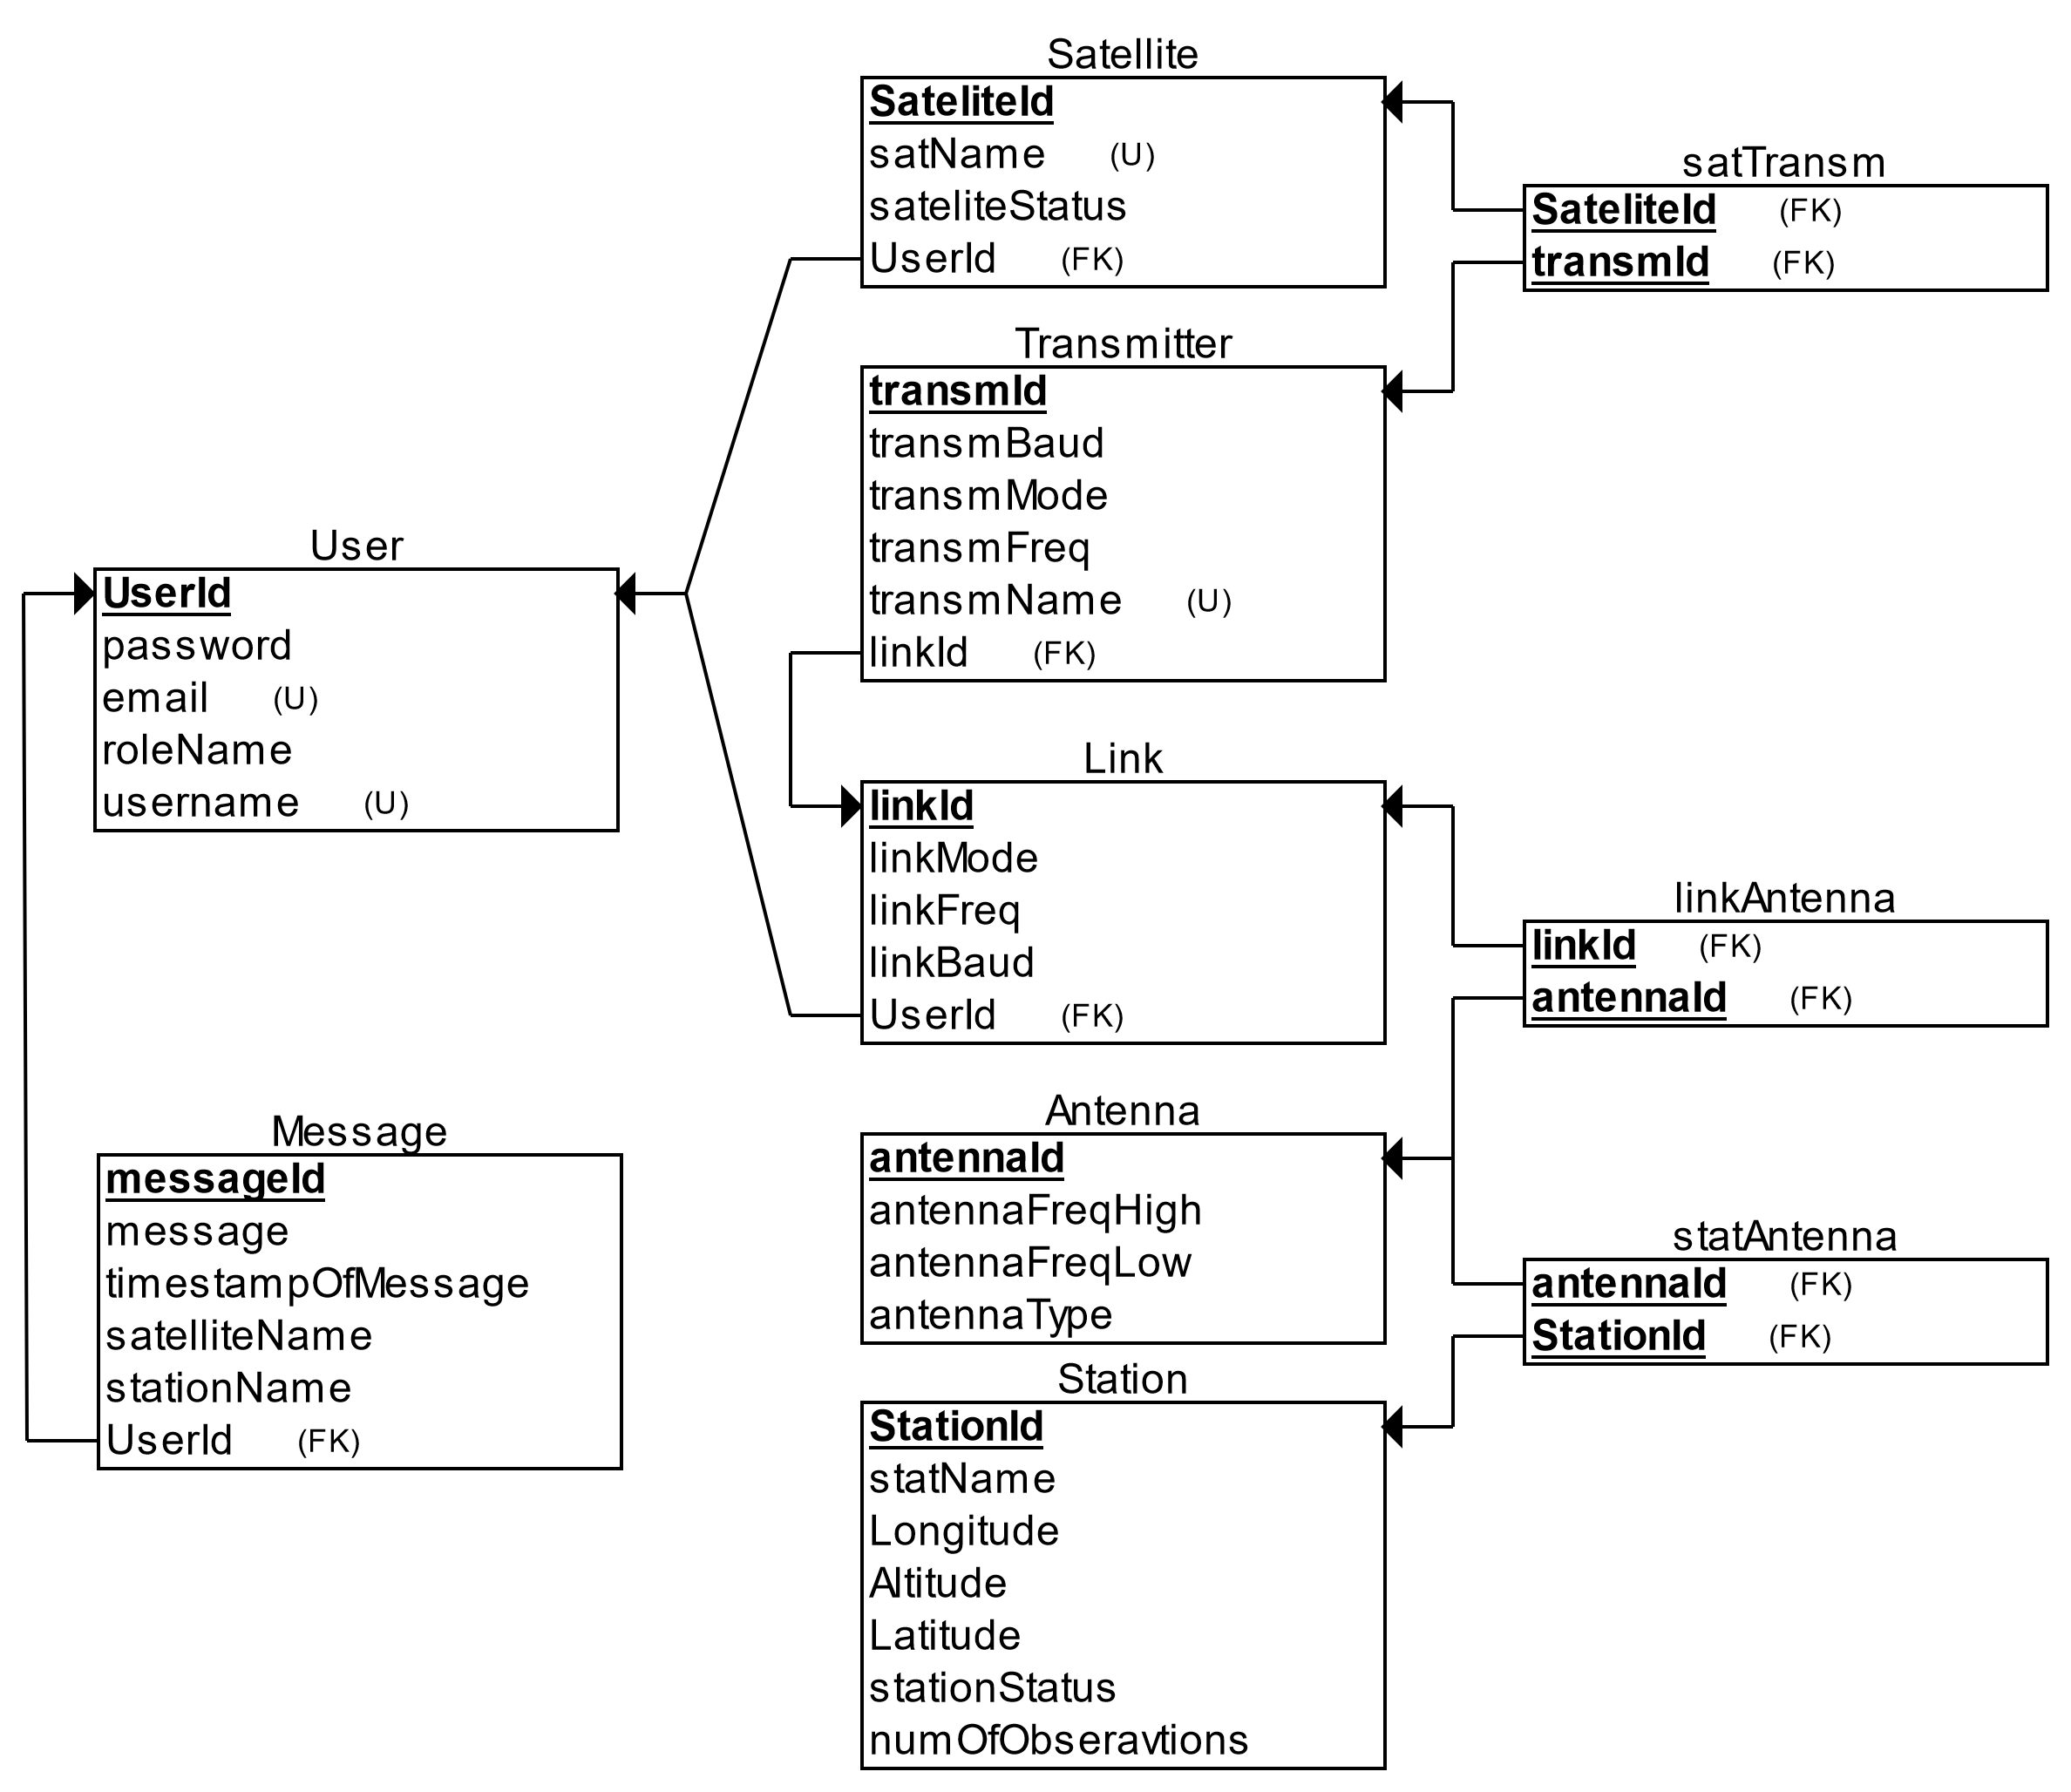
\includegraphics[width=\linewidth]{DB_Diagram.png}
					\caption{Dijagram baze podataka}
					\label{fig:Dijagram baze podataka}
				\end{figure}
			
			\eject
		\section{Dijagram razreda}
		{Na slikama \ref{fig:razredi_controllers} i \ref{fig:razredi_models} prikazani su razredi koji odgovaraju \textit{backend} dijelu MVC arhitekture. Razredi prikazani na slici \ref{fig:razredi_controllers} nasljeđuju Controller razred. Metode implementirane u tim razredima manipuliraju modelima i vraćaju zatražene podatke koji su reprezentirani modelima u listama.}
		
		
		{Model razredi preslikavaju strukturu baze podataka u aplikaciji. Razredi prikazani na \ref{fig:razredi_models} su Java klase koji predstavljaju entitete iz baze podataka. Članske varijable svake klase su atributi odgovarajućeg entiteta iz baze.}
		\begin{figure}[H]
			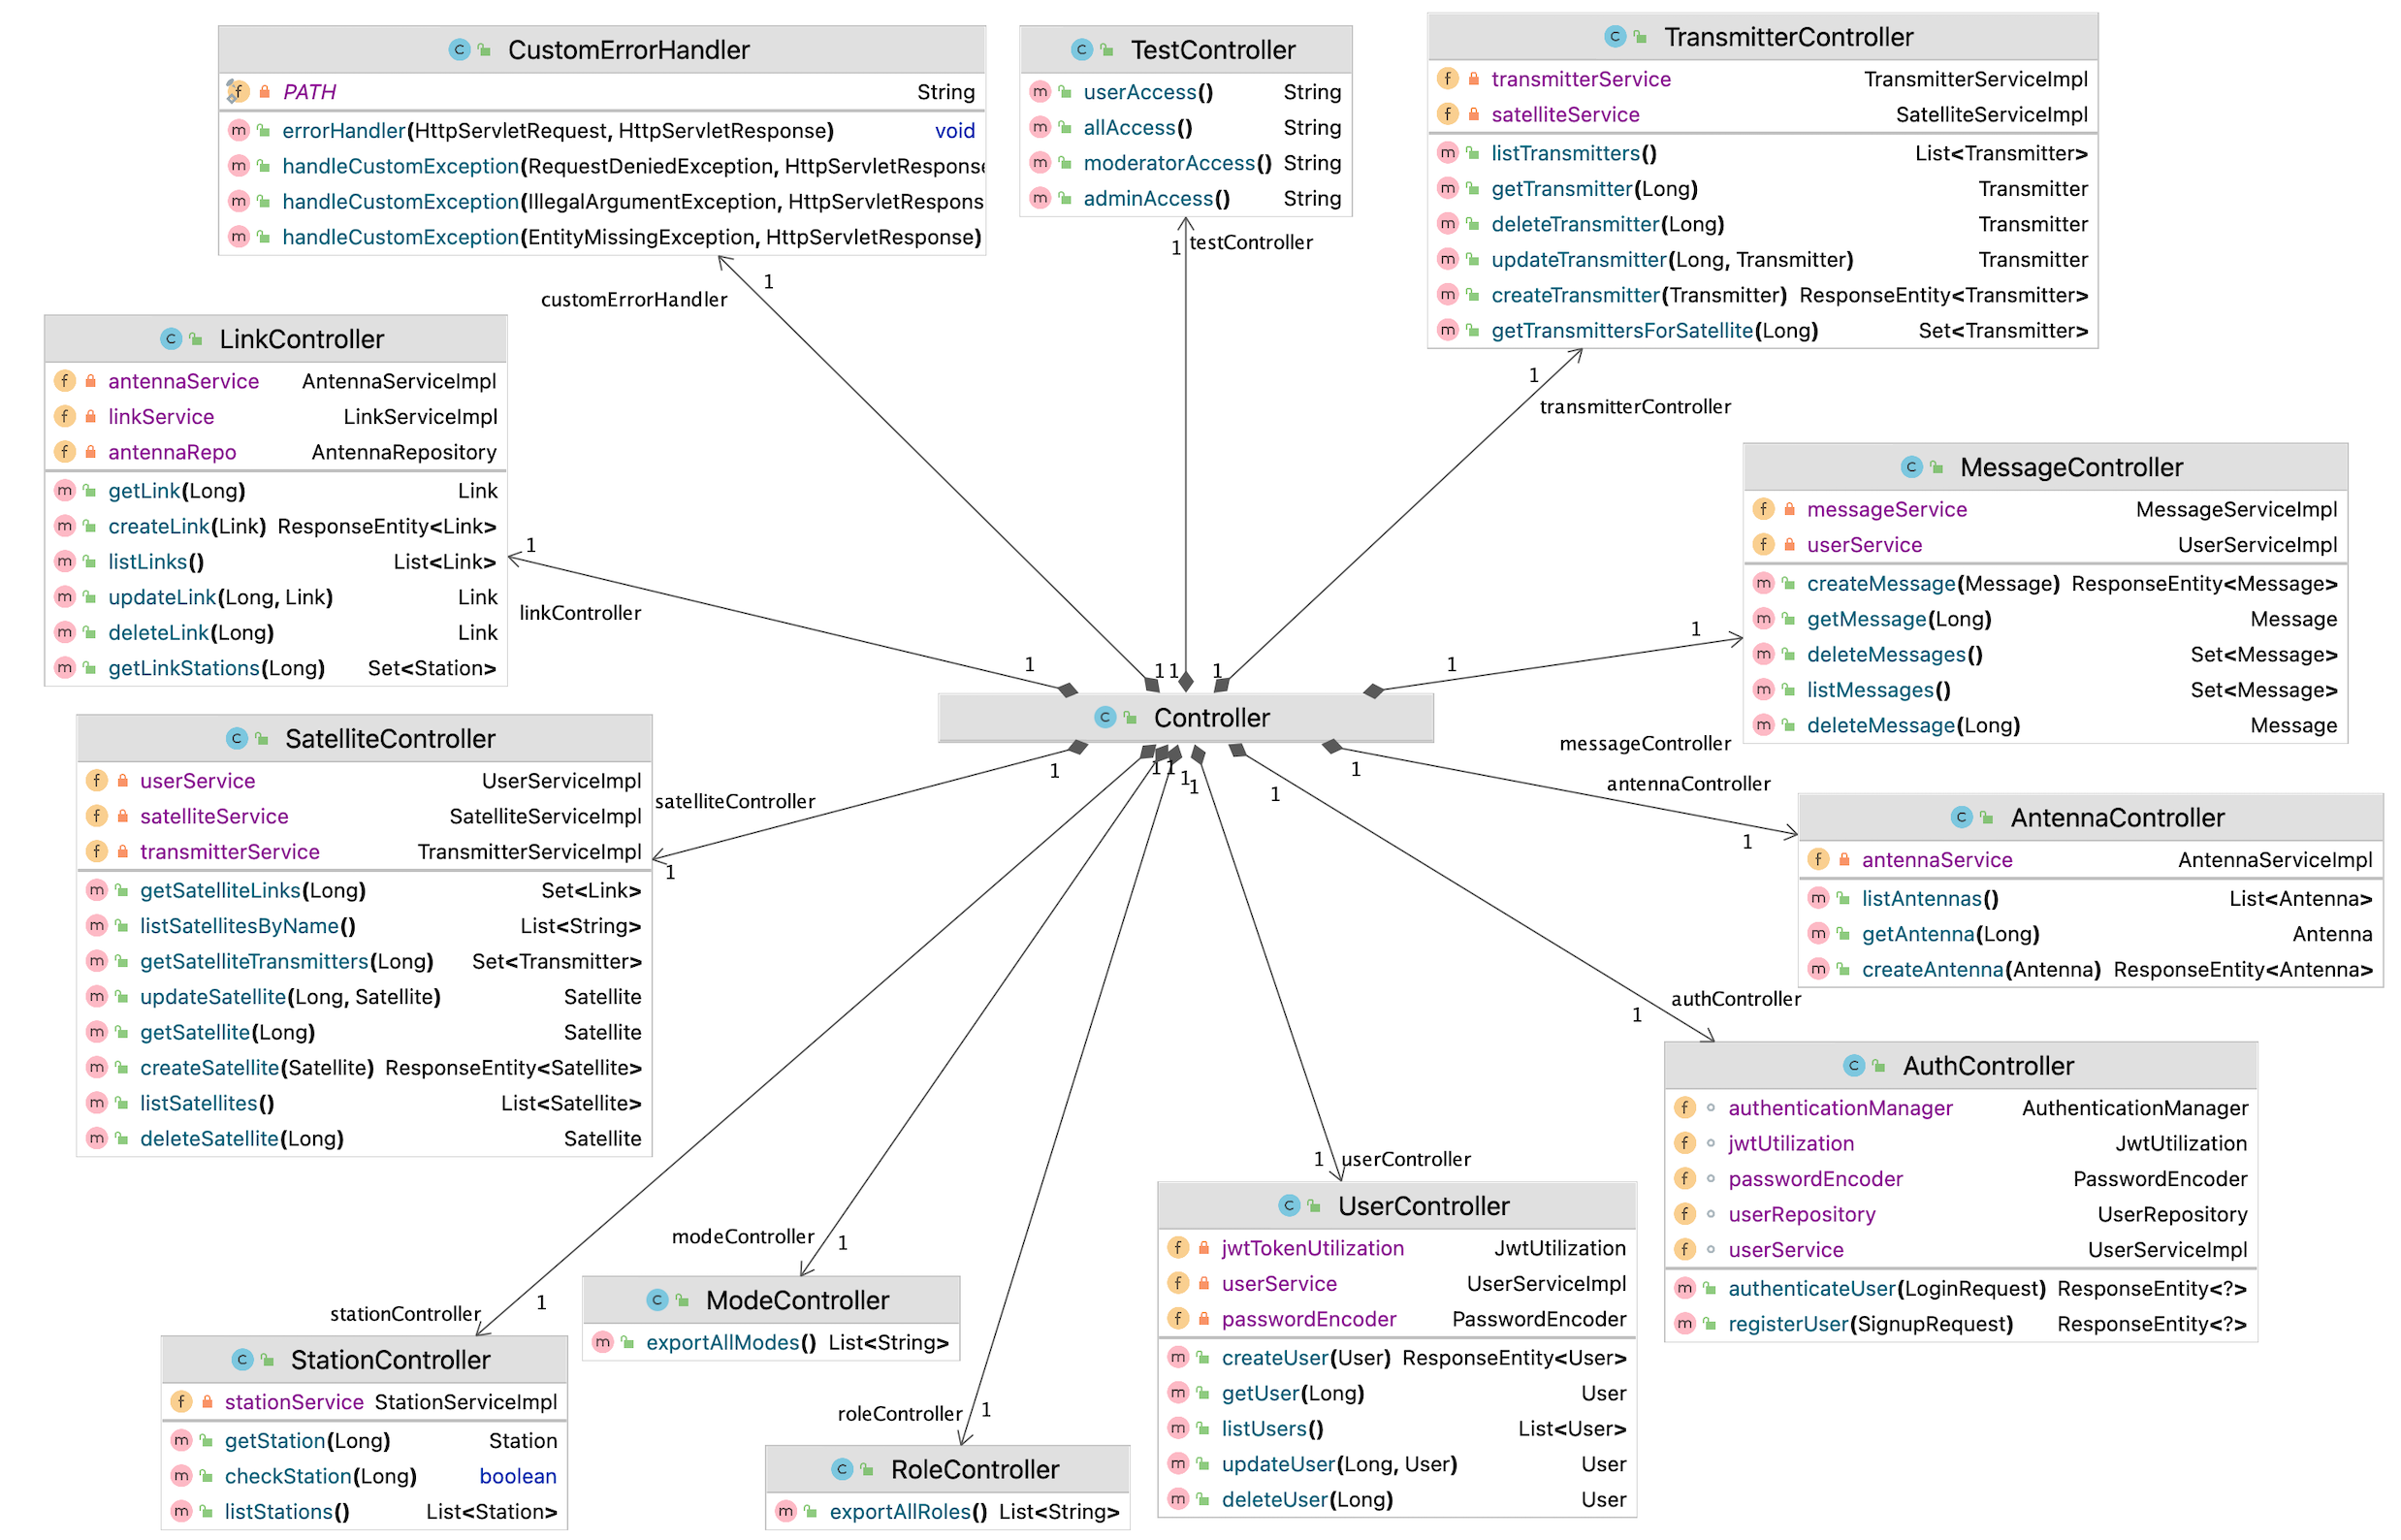
\includegraphics[width=\linewidth]{Diagram_razreda_kontrole.png}
			\caption{Dijagram razreda Controllers}
			\label{fig:razredi_controllers}
		\end{figure}
	
		\begin{figure}[H]
		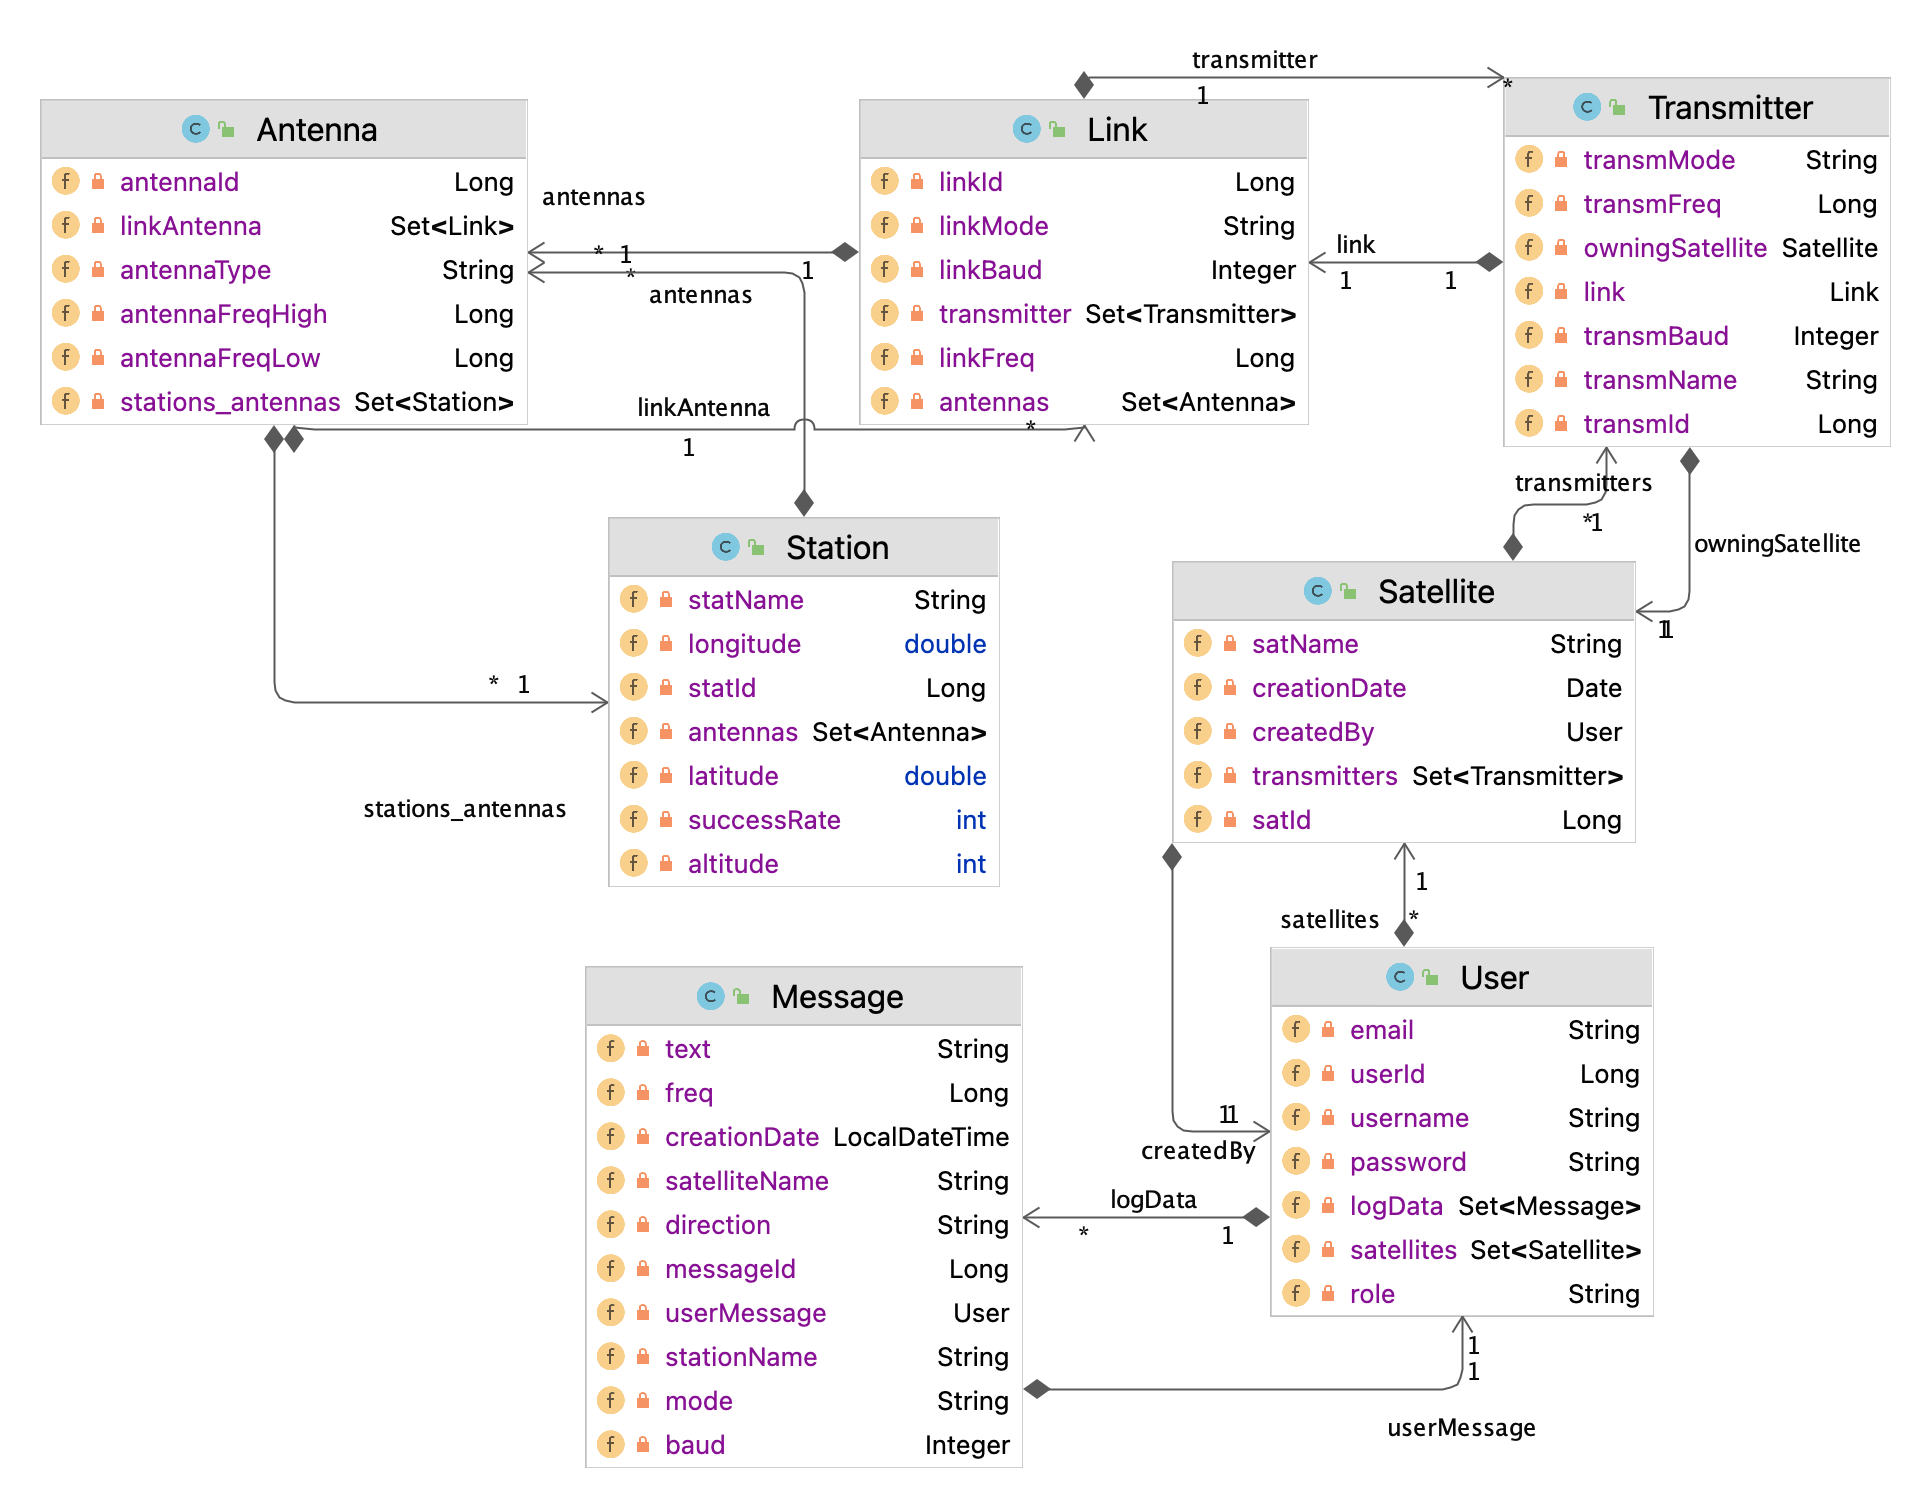
\includegraphics[width=\linewidth]{Diagram_razreda_modela.png}
		\caption{Dijagram razreda Models}
	\label{fig:razredi_models}
\end{figure}


		
		
		
		\eject
		\section{Dijagram stanja}
		
		
		{	Na slici  \ref{fig:dijagramStanja} je prikaz dijagrama stanja koji predstavlja stanja kroz koje korisnik (superadmin, admin satalita ili 
		običan korisnik) prolaze od trenutka prijave, pa sve do trenutka odjave iz web aplikacije. Početno stanje 
		za sve korisnike je prijava. Nakon prijave svim korisnicima je prikazana početna stranica "Home page" gdje se
		nalaze opcije za daljnje korištenje ovisno o ulozi.
		Svim korisnicima je zajedničko slanje poruka na prikazu "SEND MESSAGE" gdje se kroz 4 koraka odvija odabir
		satelita, odabir odgovarajučeg linka, zatim odabira načina slanja poruke te u konačnici unos poruke koja će se 
		poslati i slanje poruke. Osim slanja poruke svima je omogućen pregled povijesti poslanih poruka na prikazu 
		"MESSAGE HISTORY" gdje svaki korisnik ima mogućnost brisanja poruka iz tablice poruka. Također, svima je omogućen
		prikaz vlastitih korisničkih podataka i njihovo uređivanje.
		Superadminu je dodatno omogućena opcija dodavanje novih korisnika opcijom "Add User" te prikaz liste 
		trenutno postojećih korisnika u sustavu.
		Korisnik koji ima ulogu admin satelita je u mogućnosti obavljati CRUD akcija kreiranja (eng. create), 
		pregled postojećih podataka (eng. read), uređivanje (eng. update) i brisanje podataka (eng. delete) nad satelitima, 
		linkovima i trensmitterima.
		Zbog preglednosti na dijagramu nije dodana opcija odjava jer iz bilo kojeg prikaza se korisnik može u 
		gornjem desnom kutu odjaviti sa stranice. Također, korisnik se u bilo kojem trenutku može vratiti na početnu 
		stranicu "Home page"}
		
		

		
		
		\begin{figure}[H]
			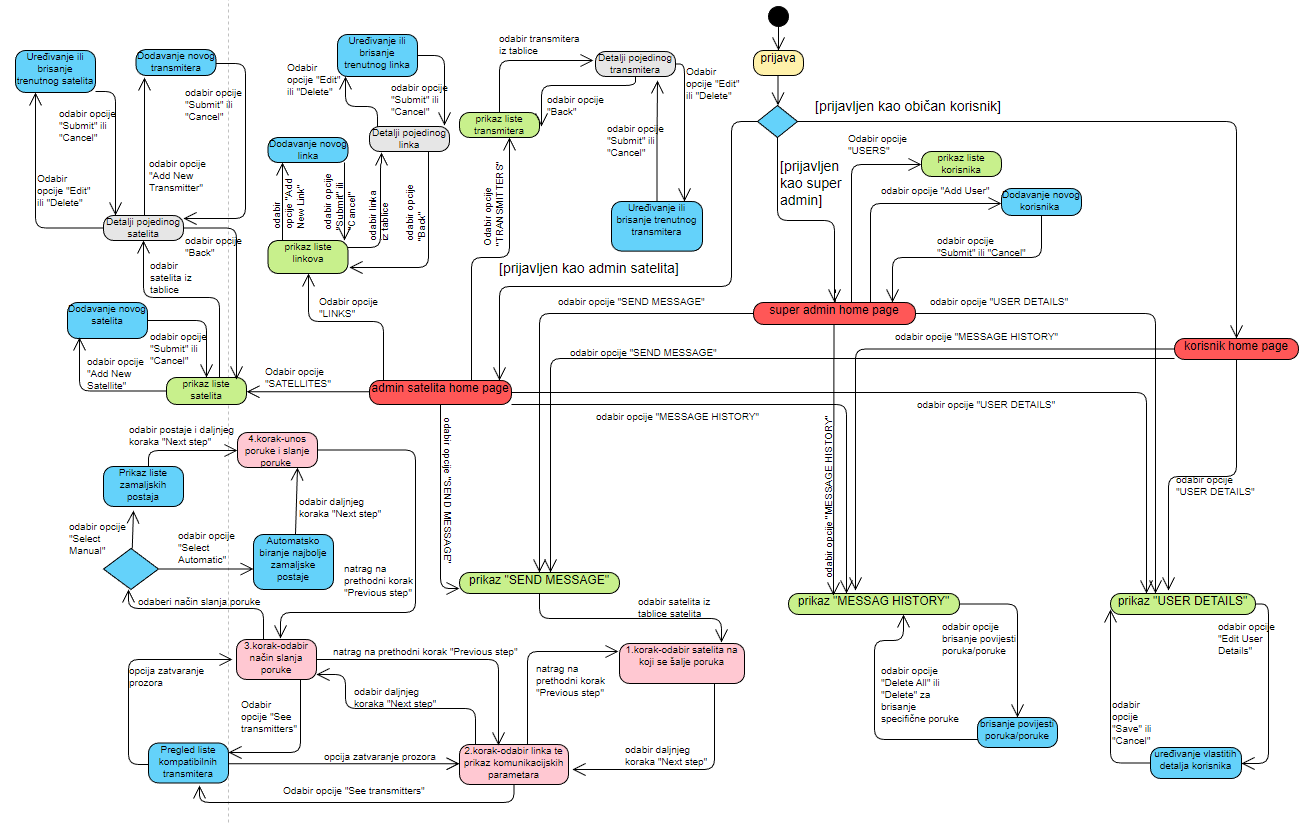
\includegraphics[width=\linewidth]{Diagram_stanja.png}
			\caption{Dijagram stanja}
			\label{fig:dijagramStanja}
		\end{figure}
		
		
		\eject 
		
		\section{Dijagram aktivnosti}
		
				\normalfont{
            Dijagram aktivnosti primjenjujemo za opise modela toka upravljanja ili toka podataka, ali ne i za modeliranje događajima poticanog ponašanja. Pri modeliranju toka upravljanja svaki korak prethodi onom sljedećem u lancu i tim se redom izvršavaju uz naglašenu jednostavnost. Na dijagramu aktivnosti prikazan na slici \ref{fig:dijagramAktivnosti} prikazan je proces slanja poruke na satelit. Prijavljeni korisnik odabire jedan od ponuđenih satelita. Sustav vraća listu kompatibilnih linkova za odabrani satelit. Korisnik zatim odabire link pomoću kojeg želi poslati poruku. Nakon što se odabere link, odabire se i način slanja poruke. Za ručni odabir, sustav vraća stanice koje mogu provesti slanje poruke na satelit uz odabrani link, korisnik zatim odabire željenu stanicu i nastavlja na sljedeći korak. Kod automatskog slanja poruke, stanicu odabire sustav prema najvećem broju obzervacija i korisnik nastavlja na sljedeći korak. Sljedeći korak je ispunjavanje forme za slanje poruke gdje korisnik upisuje željenu poruku i šalje zahtjev za slanje poruke. Kada sustav zaprimi slanje poruke, poruka se prosljeđuje na satelit server gdje se simulira odgovor satelita. Odgovor satelita i poslana poruka se spremaju u bazu podataka te se korisniku prikaže poslana poruka i primljeni odgovor. \newline}
		
		
		\begin{figure}[H]
			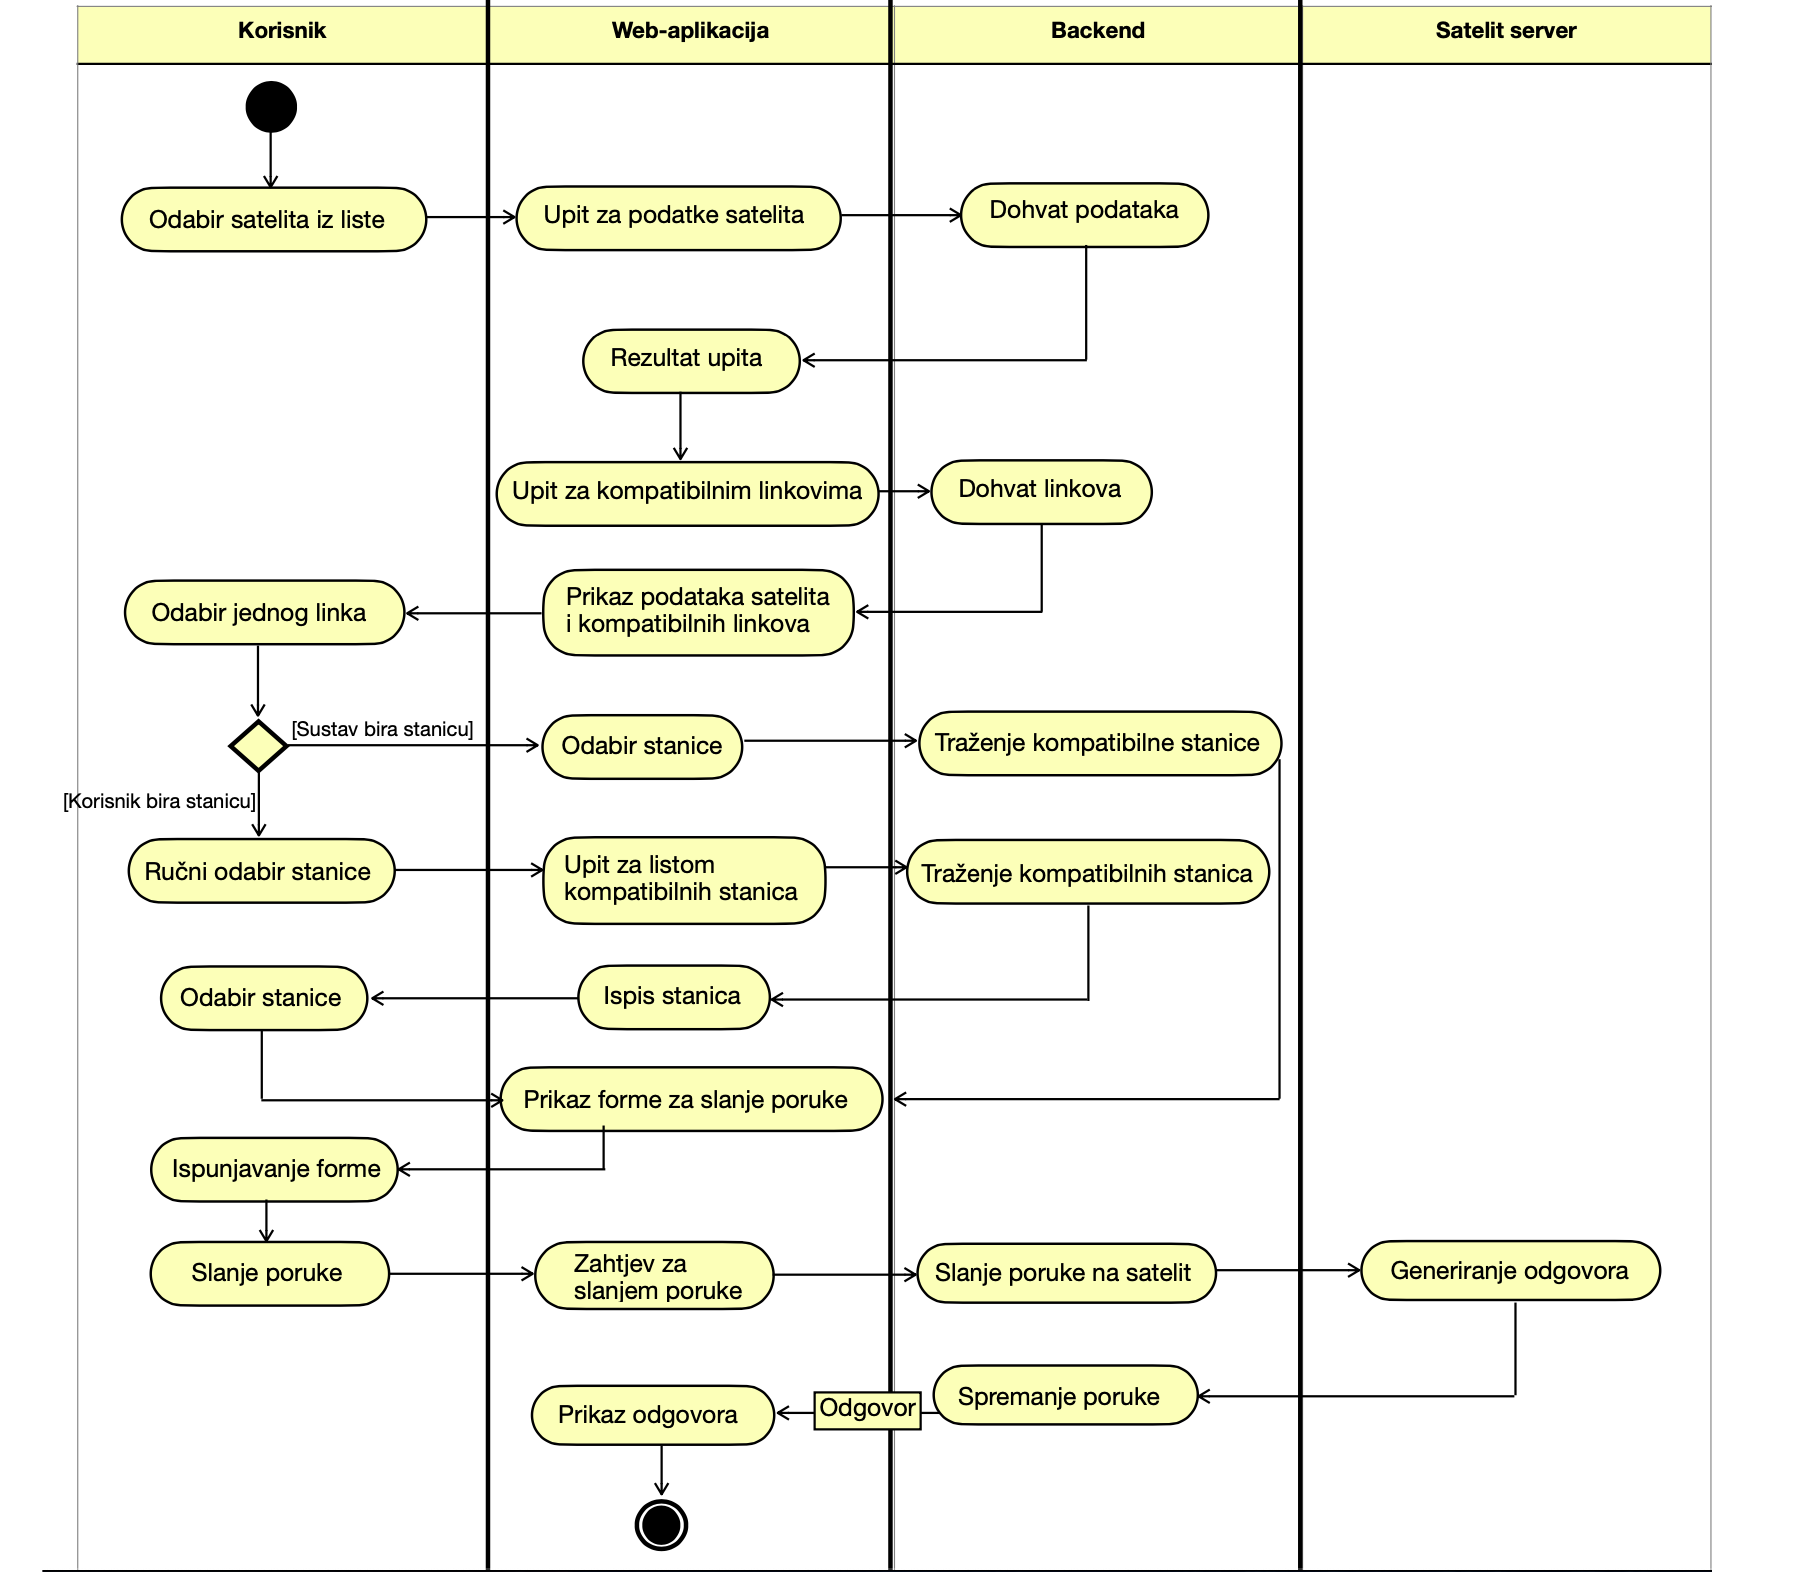
\includegraphics[width=\linewidth]{Activity_diagram.png}
			\caption{Dijagram aktivnosti}
			\label{fig:dijagramAktivnosti}
		\end{figure}
		
		\eject
		\section{Dijagram komponenti}
		
            \normalfont{
            Dijagram komponenti prikazani na slikama \ref{fig:dijagramKomponenti1} i \ref{fig:dijagramKomponenti2} opisuju međuovisnost i organizaciju i odnose u internoj strukturi. Sustavu se pristupa preko internet preglednika preko sučelja za dohvat HTML, CSS i JS datoteka koje služe za prikaz i funkcionalnost grafičkog sučelja. Router je komponenta kojom se upravlja prikaz internet stranice prema ulozi korisnika. Sučelju za primanje JSON podataka pristupa se preko REST API komponenti. Pomoću Axios biblioteke dobivene podatke s \textit{backenda} prenosimo na korisnikov preglednik. Na \textit{backendu} nam je potrebna komponenta Controllers koja služi da modele koje pretvaramo u DTO (\textit{Data transfer object}) pošaljemo na \textit{frontend} i da prenesemo odgovore sa satelita. Paket JpaRepository koristimo za pisanje i čitanje podataka iz vanjske baze podataka. Klase StationChecker i ScheduledTask koriste vansjku aplikaciju SatNOGS za najsvježije podatke potrebne za rad naše aplikacije. \newline}

		\begin{figure}[H]
			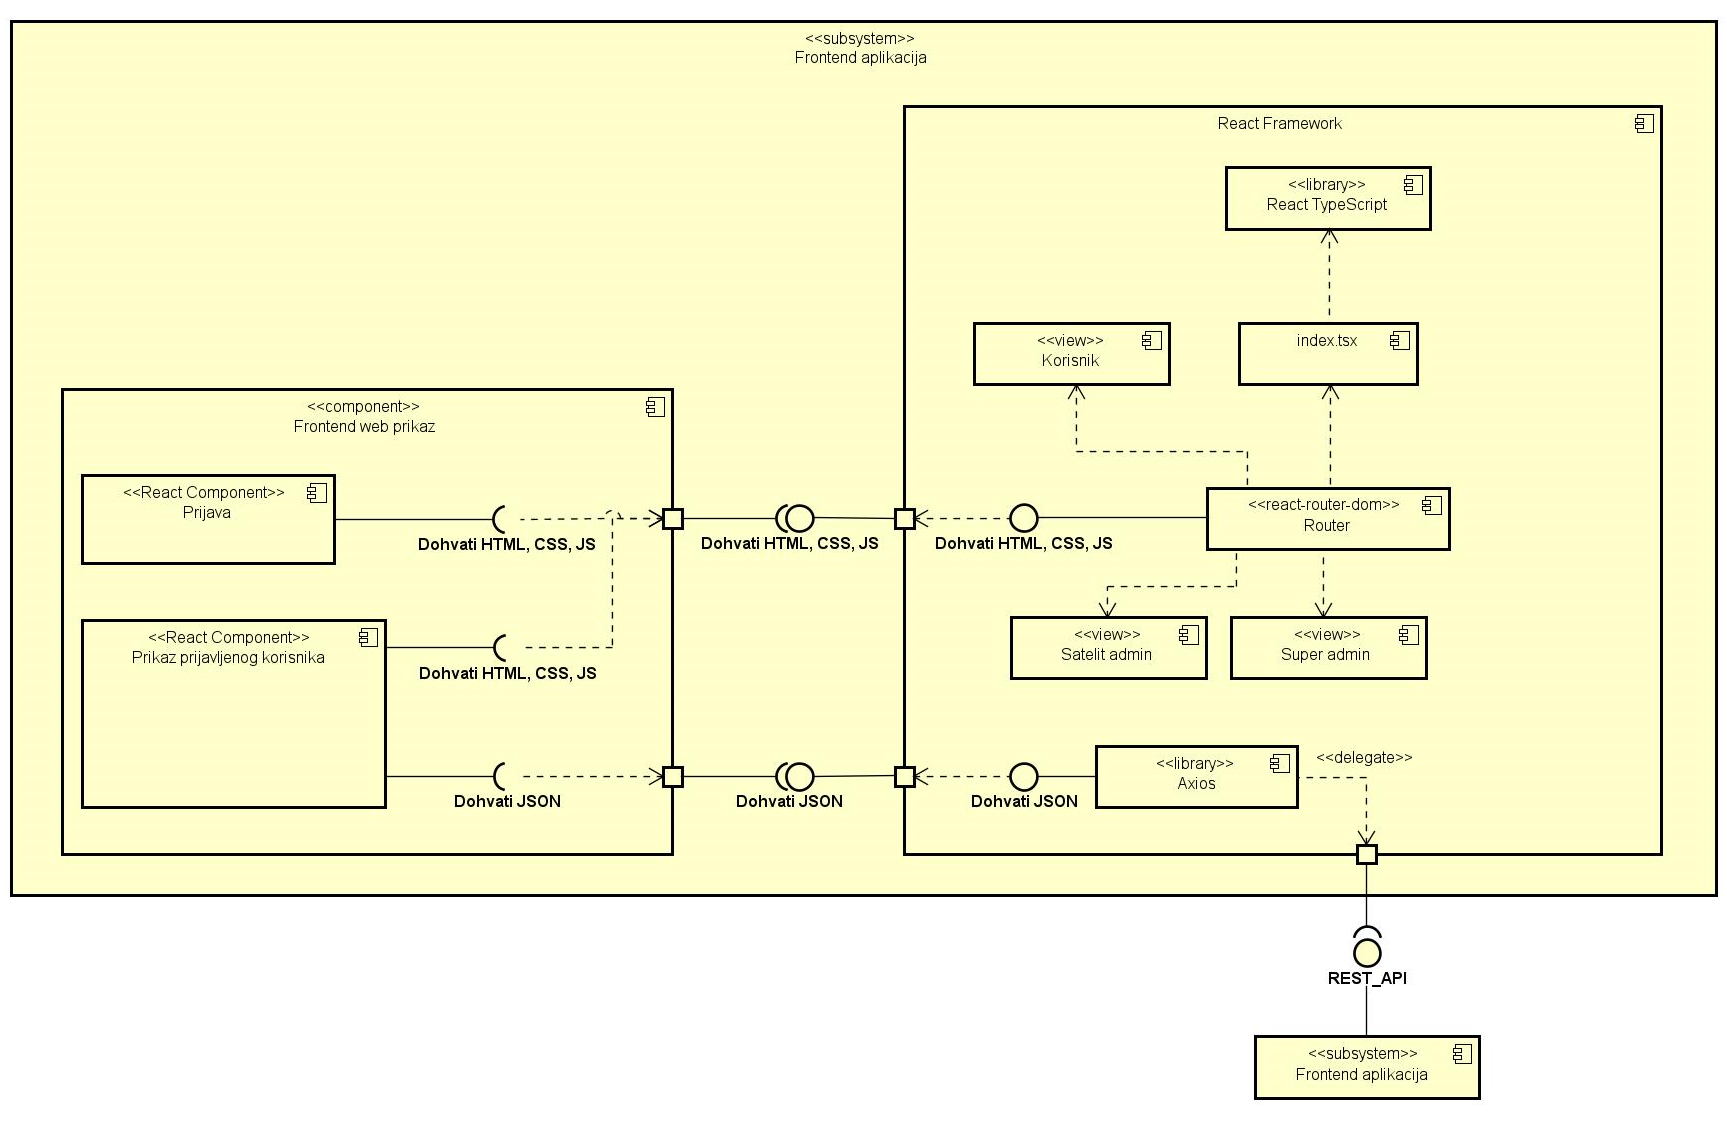
\includegraphics[width=\linewidth]{Component_diagram1.png}
			\caption{Dijagram komponenti frontend dijela aplikacije}
			\label{fig:dijagramKomponenti1}
		\end{figure}
		\begin{figure}[H]
			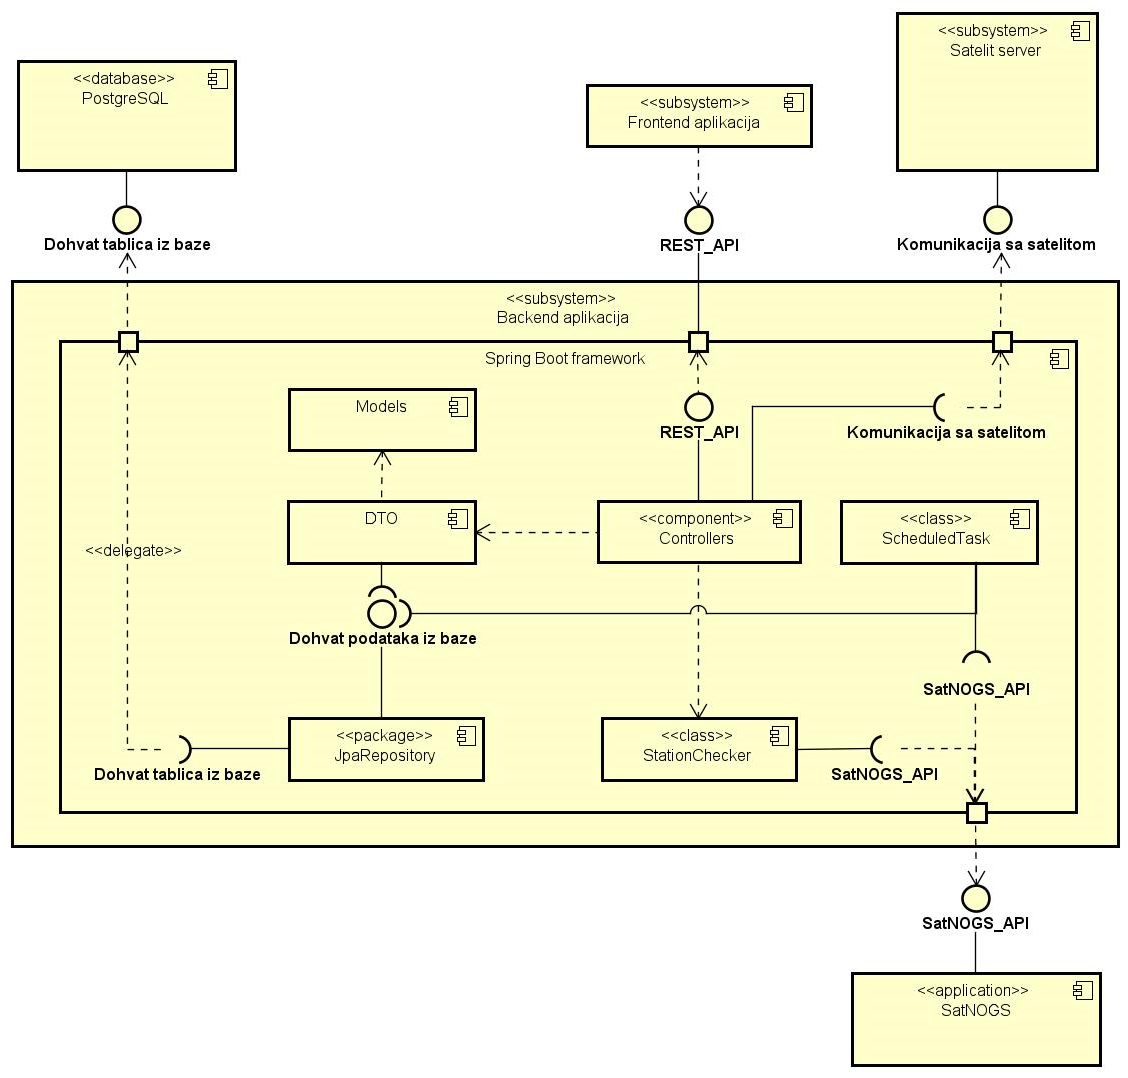
\includegraphics[width=\linewidth]{Component_diagram2.png}
			\caption{Dijagram komponenti backend dijela aplikacije}
			\label{fig:dijagramKomponenti2}
		\end{figure}